\documentclass[twocolumn,11pt]{article}
\setlength{\textheight}{9truein}
\setlength{\topmargin}{-0.9truein}
\setlength{\parindent}{0pt}
\setlength{\parskip}{10pt}
\setlength{\columnsep}{.4in}

\usepackage{amsmath,amsfonts,amssymb,amsthm,bm,caption,calc,ifthen,graphicx,url,hyperref}

\begin{document}
\pagestyle{plain}
\onecolumn
PHYS689 
\newline Homework 6
\newline Will Wainwright
\newline Repository: \href{https://github.com/wjwainwright/PHYS689}{https://github.com/wjwainwright/PHYS689}

\section*{Discussion}
This homework was pretty straight forward once I understood how to find the Nyquist frequency and how to compute the power spectrum of the FFT of the signal. I originally was unable to determine what type of signal each data set was because I neglected to subtract the mean from the signal before computing the FFT. After correcting this, I can see that N1 is pink noise. This is because it has a more gradual return to white noise from the peak corresponding to 1/f, and is much different than the sudden drop-off seen in N2. Based on the plot seen in Figure 4, I would say that the corner frequency for N1 is around 0.005 time the Nyquist frequency. I calculated the Nyquist frequency to be 500 Hz, so that means the corner frequency is 2.5 Hz. N2 appears to be a white noise signal with a sharp peak due to an added sine wave. The frequency of this peak denotes the frequency of the sine wave, which is 0.004 times the Nyquist frequency. This means that the sine wave oscillates at 2 Hz. Finally, N3 appears to be a simple white noise case, with no sharp peaks to speak of. I normalized the y-axis by dividing by N points and multiplying everything by 2 except the first and last points. I believe this is in accordance with Parseval's theorem.

\begin{figure}[!h]
	\centering
	\noindent
	\makebox[\textwidth]{
      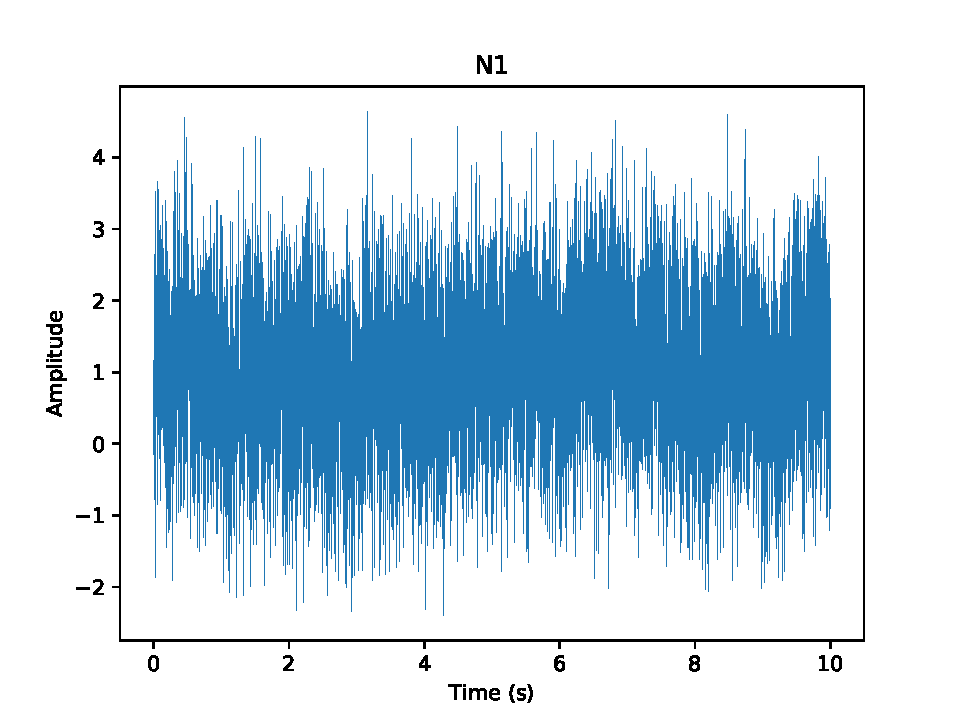
\includegraphics[width=5in]{N1_amp.pdf}}
      \caption{}
\end{figure}

\begin{figure}[!h]
	\centering
	\noindent
	\makebox[\textwidth]{
      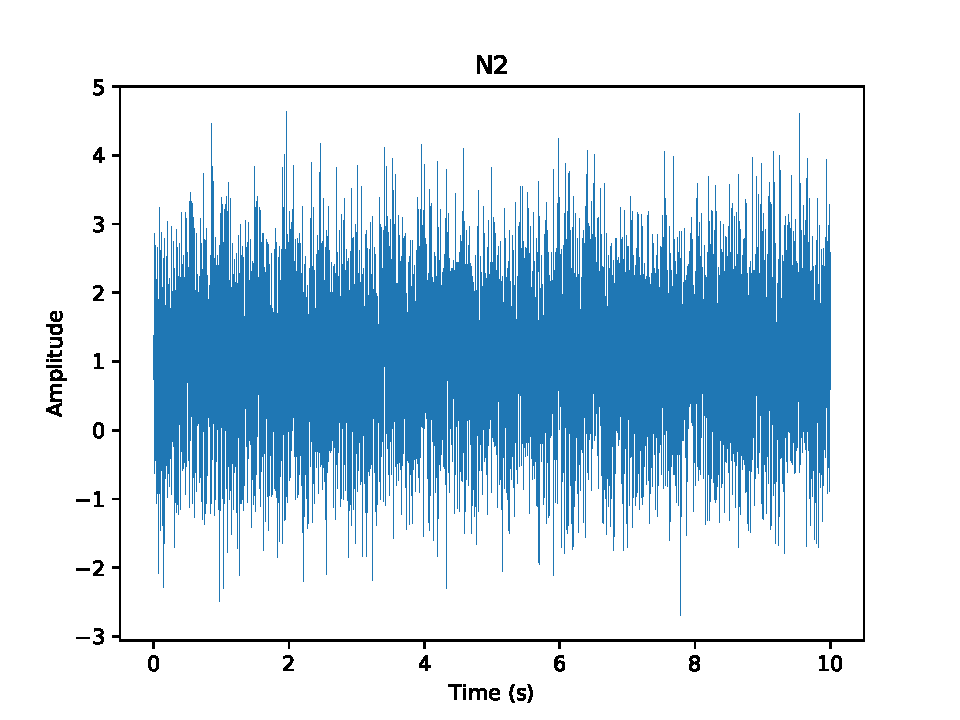
\includegraphics[width=5in]{N2_amp.pdf}}
      \caption{}
\end{figure}


\begin{figure}[!h]
	\centering
	\noindent
	\makebox[\textwidth]{
      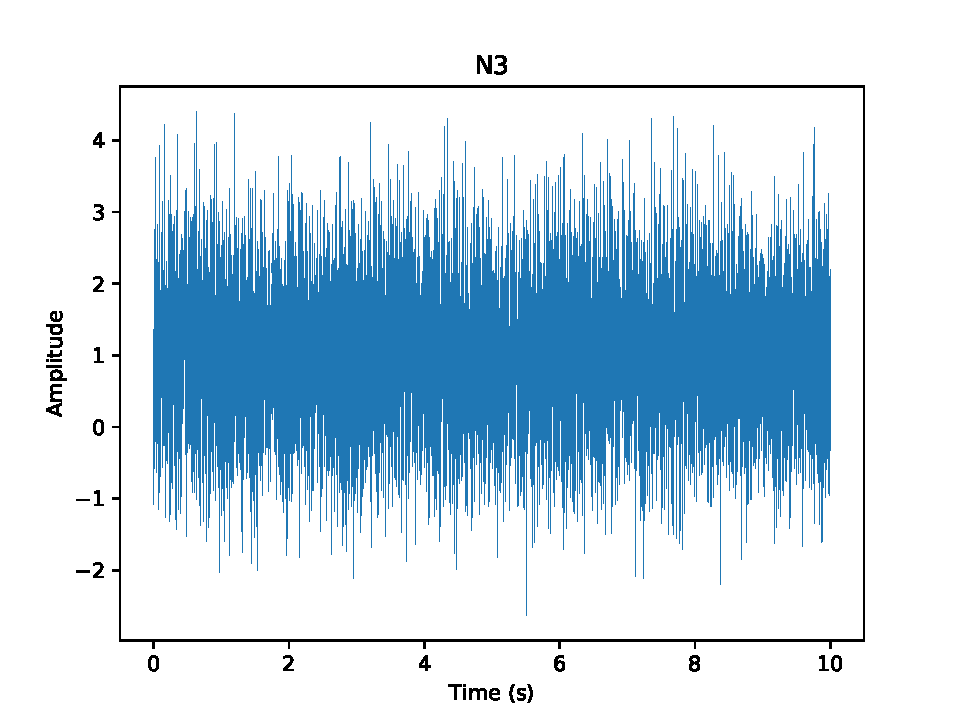
\includegraphics[width=5in]{N3_amp.pdf}}
      \caption{}
\end{figure}

\begin{figure}[!h]
	\centering
	\noindent
	\makebox[\textwidth]{
      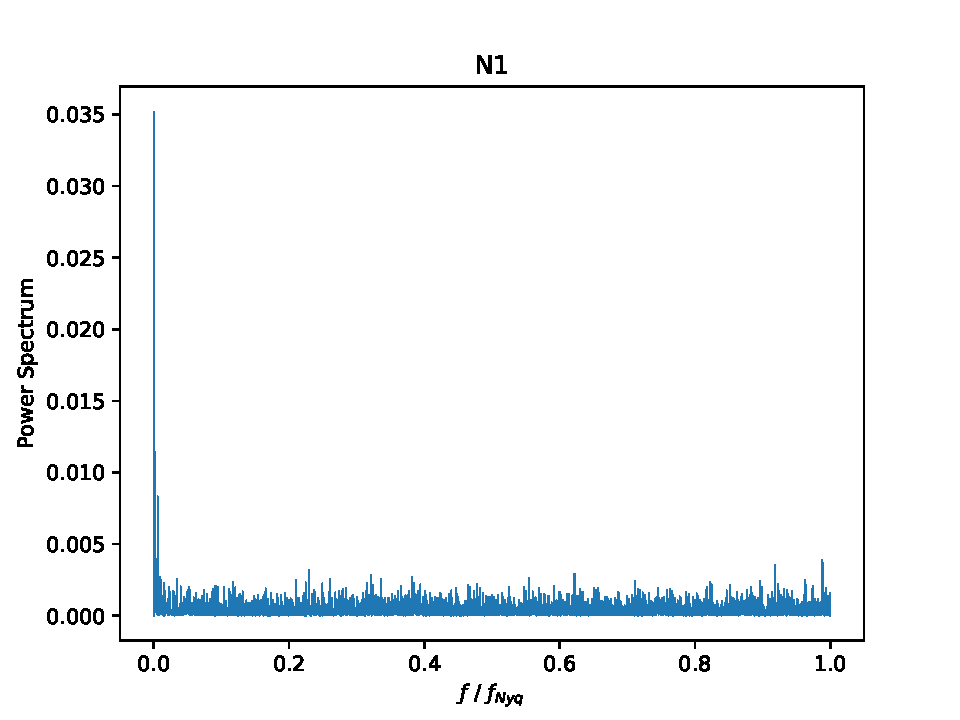
\includegraphics[width=5in]{N1_fft.pdf}}
      \caption{Power series of the FFT for N1. This signal is pink noise, as can be seen by the curved drop from the peak to white noise. The knee frequency is around 0.005 times the Nyquist frequency.}
\end{figure}

\begin{figure}[!h]
	\centering
	\noindent
	\makebox[\textwidth]{
      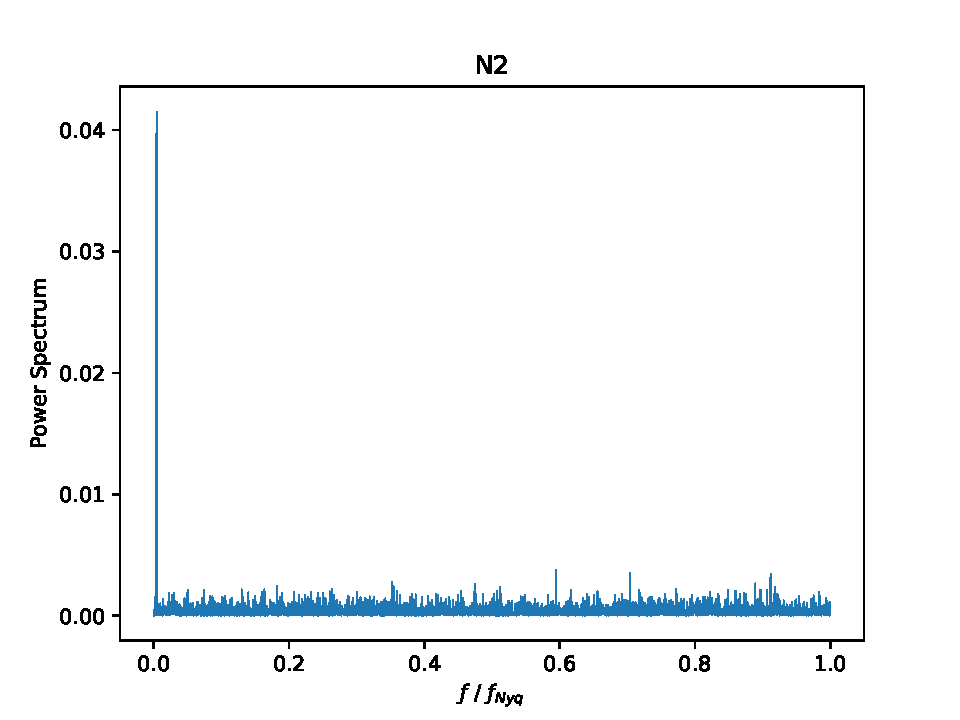
\includegraphics[width=5in]{N2_fft.pdf}}
      \caption{Power series of the FFT for N2. The large spike in the signal and then immediate return to white noise makes apparent that there is a sinusoidal signal added into regular white noise. Based on the peak, the sine wave has a frequency of 0.004 times the Nyquist frequency.}
\end{figure}

\begin{figure}[!h]
	\centering
	\noindent
	\makebox[\textwidth]{
      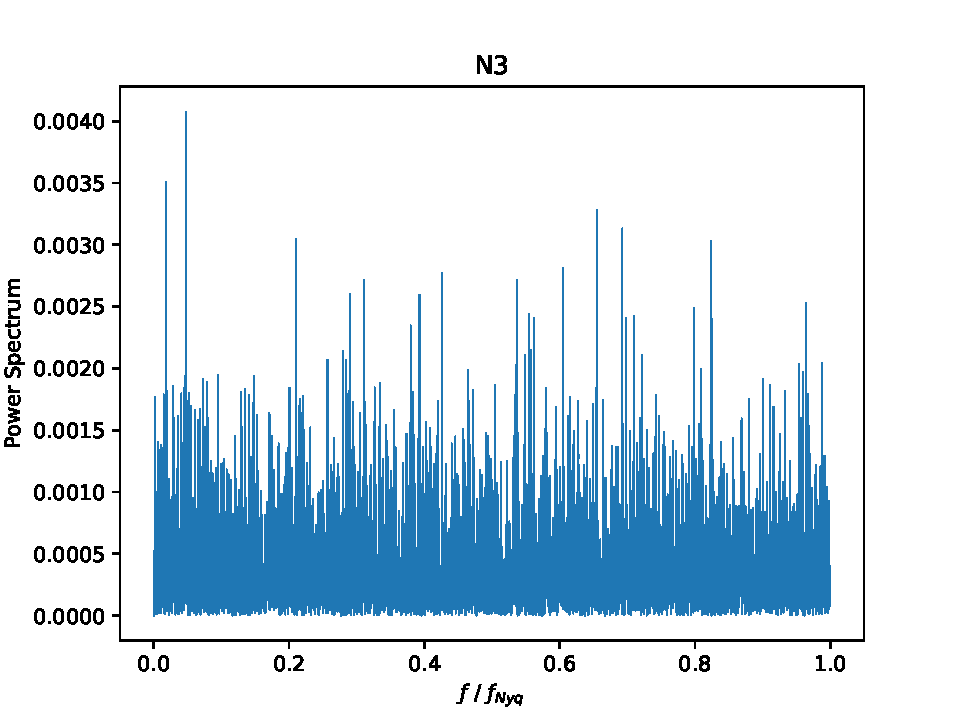
\includegraphics[width=5in]{N3_fft.pdf}}
      \caption{Power series of the FFT for N3. Nothing too special going on here, just white noise.}
\end{figure}


\end{document}